\chapter{Introduction}

%World leaders adopted the seventeen Sustainable Development Goals stated by the United Nations (UN) in 2015. One of the Goals (SDG2) is pointed at a major challenge the world faces; End Hungry. Currently 815 million people suffer from the effects of hunger. In 2050 it is prospected 10 billion people are living on earth. On a world-wide scale thorough changes in the agricultural system are needed to guaranty food security for all (Bron: SDG 2). \\

%Sustainable Development Goal number two (SDG2), as one of the seventeen SDGs stated by the United Nations in 2015, is pointed at a major challenge the world faces; End Hungry. Currently, 815 million out of the 7,5 billion people on earth suffer from hunger. It is likely these numbers will increase by looking at growth prospects (world population of 10 billion people in 2050). Thorough global agricultural system changes are needed to guaranty food security for all, now and in the future (Bron: SDG 2). The availability of water is inseparable to this process. Agricultural irrigation alone covers about 70 per cent of the entire sociatal water use (bron). \\

%Agricultural irrigation alone covers about 70 per cent of the entire humanitarian fresh water use. Water for food production needs to be accounted (bron). 

%'Ending Hunger' is one of the Sustainable Development Goals (SDG2) stated by the United Nations in 2015. Currently, 815 million out of the 7,5 billion people on earth suffer from hunger. By looking at growth projections (world population of 10 billion people in 2050) future expansion is likely. Thorough global agricultural system changes are needed to guaranty food security for all, now and in the future (Bron: SDG 2). The UN Food and Agricultural Organisation (FAO) predicts the global food production needs to be doubled in 2050. Due to strong patterns of urbanization and changes in diets these necessities can be even higher in (among others) Sub-Saharan Africa (SSA). \\

%
%innovative smallholder farmers (bottum-up). The governement of the Netherlands for example facilitates innovative   implementation of resource efficient production techniques. The government of the Netherlands envisages a significant role for semi   role  hier ziet de nederlandse overheid een voorname rol weggelegd voor smallholder farmers. 
%
%
%Smallholder farmers can bridge the gap by the implementation of improved techniques improve their production process productProcess improvement and Implementation of innovations by smallholder farmers are for example supported by the government of the Netherlands in the Small Business Innovation Research (SBIR) call (bron).   

%Increased food demands puts pressure on SSA natural resources. At the same time the local agro-food sector can make a virtue of this inevitability (bron). Implementation of resource efficient production techniques can bridge the gap between actual and potential agricultural yields. 

%Dependent on (higher) latitude the wet season can be shorter and more intense (bron: Hap).

'End Hunger' is one of the Sustainable Development Goals stated by the United Nations \citep{UnitedNations2018}. Currently, 815 million people on earth suffer from hunger. In coherence with the prospects of the world population (growth up-to 10 billion people by the year 2050) hunger is likely to expand \citep{UnitedNations2018}. The UN Food and Agricultural Organisation (FAO) expects a needed doubling of the global food production \citep{FAO2018}. Due to strong patterns of urbanization and changing diets the nutrition necessities are even higher in (among others) Sub-Saharan Africa (SSA). Local agricultural sectors within SSA can make a virtue of the inevitable rising food demands \citep{MinistryofForeignAffairs2018}. The present gap between the actual and potential yield can be bridged by small-scale agricultural innovations. Smallholder farmers can increase productivities by the implementation of more resource-efficient techniques. This bottom-up development approach is for example supported by the government of the Netherlands (SBIR program) \citep{MinistryofForeignAffairs2018}. \\ 

Water availability is of key interest in food production. 70 percent of the entire humanitarian fresh water-use serves agricultural purposes \citep{UnitedNations2014}. Within SSA, the northern Ghana region encounters favourable agricultural climatological conditions (semi-arid). The Ghana Meteorological Services Department (MSD) measured (1971-2007) annual average precipitation of 800-1250 mm/y \citep{HAP2011}. In absolute terms, satisfying water quantities to become self-sufficient in food supply \citep{MinistryofForeignAffairs2018}. However, precipitation is unevenly spread over the year. The utmost extent of annual precipitation is typically covered by four months of wet season (late May - October). As a consequence, northern Ghana is subjected to both seasonal flooding and long periods of drought (Figure \ref{fig:Flood_Drought}). \\
%
%Bron: rijksdienst voor onder
%wereldwijd probleem.. in 2050 moeten 10 miljard mensen gevoed kunnen worden. gevolgen klimaatverandering brengt de mondiale landbouwproductie in gevaar. door droogte en overstroming juist niet veel meer landbouwgrond beschikbaar. daarom deste belangrijker om huidige mogelijkheden te verbereren. 
%
%Het is dus een wereldwjd probleem maar in sub-sahara africa nog gevoeliger. In afrika de stijgende vraag naar voedsel ver boven wereld gemiddelde (verwachting 4x wat er nu is, is nodig in 2050 in afrika). 
%
%Sub-Sahara afrika heeft potentieel, maar wordt nu niet optimaal gebruikt. Ook wordt er al een groot beslag gelegd op natuurlijke hulpbronnen. SBIr heeft een prijsvraag gericht op oplossingen voor kleine en middelgrootte boeren, het moet bestendig zijn tegen klimaat verandering, ecologisch houdbaar en  moet zorgen voor locale werkgelegenheid. 
%
%SBIR: 
%een van de randvoorwaarden voor jou idee: -verhogen (kwanliteit, maar ook) quanrtititeit. oftewel het moet de productiviteit omhoog brengen. Daar doen ze een oproep op voor een idee. 
%-En het moet van toepassing zijn op sub-saharan africa. oftewel bijvoorbeeld ghana.  

\begin{figure}[h!]
	\centering
	\begin{subfigure}[b]{0.5\linewidth}
		\centering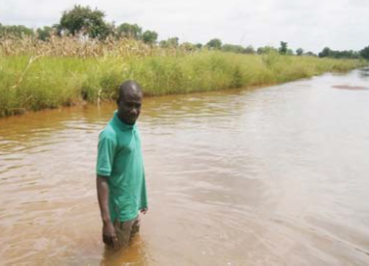
\includegraphics[width=0.9\linewidth]{Flood}
		\captionsetup{justification=centering}		
		\caption{\label{fig:Flood}}
		\end{subfigure}%\hfill
	\begin{subfigure}[b]{0.5\linewidth}
        \centering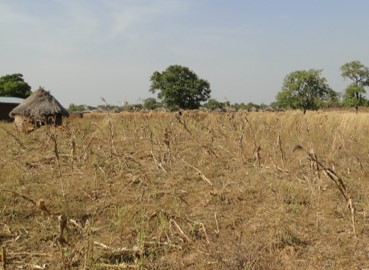
\includegraphics[width=0.9\linewidth]{Drought}
		\captionsetup{justification=centering}		
		\caption{\label{fig:Drought}}
		\end{subfigure}
		\captionsetup{justification=centering}	
	\caption[Example on (\subref{fig:Flood}) flood near Weisi, Upper West Region and (\subref{fig:Drought}) drought near Nungo, Upper East Region]{Example on (\subref{fig:Flood}) flood near Weisi, Upper West Region (source: \citep{Owusu2017} and (\subref{fig:Drought}) drought near Nungo, Upper East Region} 
	\label{fig:Flood_Drought}
\end{figure}

Northern Ghana's food production is predominantly cultivated during the wet season. Dry season (irrigation based) agriculture takes place at small-scale. Only restricted quantities of groundwater are used in the irrigation process. Currently,  local groundwater use is estimated to be approximately 5\% of the annual recharge (2.5-10\% of annual precipitation) \citep{Martin2008}. The amount of water withdrawn is marginal and the environment is self-reliant. However, climate change can potentially have a negative influence. Natural recharge can become lower, while governmental policies are more and more pointed at the intensification of dry season agriculture \citep{Wood2013}. In the near future, it is possible that discharge rates will exceed natural recharge and groundwater extraction is no longer sustainable. Managed Aquifer Recharge (MAR) can potentially contribute to the continued sustainable use of groundwater in northern Ghana. \\ 


%Cropping activities are preferably extended in time (dry season) to anticipate on rising food demands. Use of abundant (wet season) flood water by temporary surface storage is a hand on solution. However, calculated potential evaporation rates (MSD) transcend measured average annual precipitation (bron, HAP). As an alternative in dry season water availability extraction of groundwater is applied. 
%
%Wet season rain-fed crop growth 
%Om droogte tegen te gaan zaak om overtollig water vast te houden. maar dat is nog niet zo makkelijk. bovengrond 
%calculated potential evaporation rates exceed annual average rainfall. Therefore surface water storage is not desirable (HAP). Als alternatief kan uitgeweken worden naar subsurface. 
%
%een van de innovaties (eerder benoemd) ligt mogelijk bij improvements of ASR-system. 
%Water is of a key aspect in  
%
%\section{Background}
%Ghana background. uiteindelijk zonder kopje!
%vertel kort over ghana regenseizoen, droge seizoen etc. hoe de landbouw daar nu uit ziet. welke producten. in welke periode verbouwd. etc. 
%zeg dat omstandigheden er zo zijn dat water niet zo maar kan worden opgeslagen bovengronds. climate. (plus bron). 
%
%vervolgens over hoe de small scale landbouw daar van water wordt voorzien. 
%Werking van het asr systeem. 
%dat de werking nu nog niet toereikend is. of dat er echter meer uit het systeem gehaal kan worden. nu landbouw voor bijvoorbeeld een acre maar men wil wel naar bijvoorbeeld een hectare. (5 maal zo intensief). 
%Vertel ook dat het hier om dry season verbouwing gaat. en dat er hierdoor kan worden afgeweken van gewone gewassen. 
%
%Door het klimaat kan niet altijd efficient water bovengrons worden vastgehouden. 
%Alternatief is MAR. heel veel verschillende vormen. zoek bron. 

\textbf{Aquifer Storage \& Recovery (ASR) systems}\\
Water entering a catchment (e.g. precipitation, river or groundwater flow) partially and temporarily contributes to local recharge of groundwater \citep{Fitts2012}. The natural water cycle can be manipulated by human interventions. Temporarily available water can be added to the subsurface by the creation of preferential flow paths; Managed Aquifer Recharge (MAR) \citep{Dillon2009}. Different objectives can induce the implementation of MAR. One can think of underground water storage to reduce flooding or to counter groundwater shortages. Moreover, implementation can be beneficial for the local retention of water. MAR applications reduce water losses through evaporation and run-off. \\

MAR concepts exist in wide varieties, e.g. surface infiltration basins and sand dams \citep{Dillon2009}. A particular MAR type takes central stage in this research; Aquifer Storage and Recovery (ASR) systems. Besides the basic MAR principle, groundwater recharge, ASR systems are designed for groundwater withdrawal as well. The principle functions of an ASR system are visualized in Figure \ref{fig:ASR}.

\begin{figure}[h]
 \centering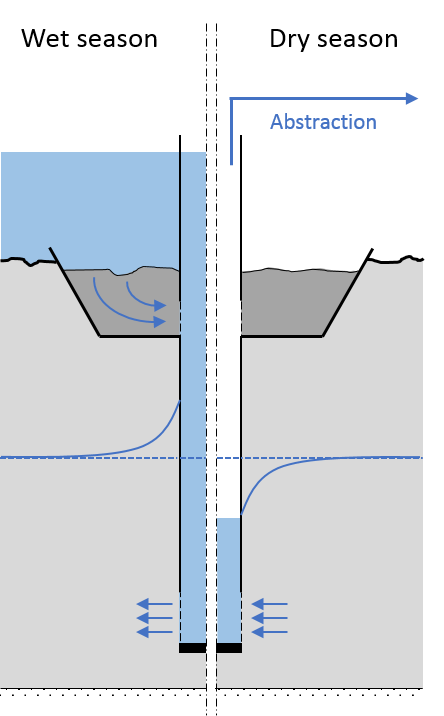
\includegraphics[width=0.33\linewidth]{Wet_Dry}
 \captionsetup{justification=centering}
 \caption{The year-round principal functions of an Aquifer Storage \& Recovery (ASR) system}
 \label{fig:ASR}
\end{figure}

An ASR system offers a solution when natural surface infiltration characteristics are insufficient. Wet season water surpluses (e.g. flood and inundation) can be stored in the subsurface by the use of an ASR system. Flood water enters the system under gravity. An infiltration bed around the borehole serves as the preferential path of flow. For purification purposes the bed is designed with a specific soil arrangement \citep{Owusu2017}. Dependent on borehole screen depth the ASR system can be connected to shallow (unconfined) and/or deeper ground layers (unconfined/confined). Dry season water withdrawal takes place by the installation of a submergence pump. \\

%\textbf{Research purposes} \\
\textbf{Research questions} \\
Northern Ghana based ASR systems make use of locally available natural resources. The system acts as a seasonal bridge, it converts flood water into irrigation water. In the northern Ghana context, the ASR system relation to absolute water volumes is undetermined (e.g. impact on local nature and agricultural benefits). From a sustainable point of view it is desirable to gain knowledge on year-round ratios between groundwater recharge (wet season) and discharge (dry season). Furthermore, northern Ghana smallholder farmers can potentially benefit from increased system efficiencies (Figure \ref{fig:Purpose_Multi}). A desired development in the process of becoming a (more) self-sufficient food region. However, the impacts of ASR system innovations are undiscovered. Objective of this research is to conduct a feasibility study on sustainable use of a synthetic ASR system in northern Ghana; taking present conditions and multiple system improvements into account. This research aims to answer the following research question: \\

%
%However, ASR system innovations to potentially increase efficiencies in the use of natural resources are undiscovered within the northern Ghana context.

%\textbf{How can Aquifer Storage and Recovery (ASR) system improvements be beneficial for the availability and sustainable use of groundwater in northern Ghana small-scale agriculture?} \\

%\textbf{How can modifications of Aquifer Storage and Recovery (ASR) systems improve the availability and sustainable use of groundwater in northern Ghana small-scale agriculture?} \\

\textbf{How can Aquifer Storage and Recovery (ASR) systems be improved to increase the availability and sustainable use of groundwater in northern Ghana small-scale agriculture?} \\

\begin{figure}[h]
 \centering
\includegraphics[width=0.8\linewidth]{Purpose_Multi}
 \captionsetup{justification=centering}
 \caption[A simplified visualization of the desired results of ASR-system improvements]{A simplified visualization of the desired results of ASR-system improvements (At present a single poly tank is filled on daily dry season bases). (visual support by Housin Aziz, Jhun Capaya and Nibras@design from Noun Project - \url{https://thenounproject.com})}
 \label{fig:Purpose_Multi}
\end{figure}

The main research question can be solved in consecutive parts. Three addition research question are stated that have to be answered:

\begin{itemize}
\item{\textit{Which range of values for transmissivity ($T$) and storativity ($S$) can be obtained from aquifer tests applied at multiple study sites in northern Ghana?}
\smallskip \\
It might seem trivial, but the functioning of an ASR system is dependent on its surroundings. Locally applicable geohydrological parameters ($T$ and $S$) have to be determined for the research follow-ups. The desired information is obtained by the application of site-specific measurements at multiple locations within northern Ghana.} 
\end{itemize} 
%The Fieldwork set-up strategies as well as the approaches in data analysis are included in the methodology (Section \ref{section:Methods_fieldwork}). The answers to the sub-question are generated in Chapter \ref{chapter:Fieldwork_data_analysis}.

\begin{itemize} 
%\item{\textit{How and to what extent can ASR system improvements gain groundwater discharge rates, while maintaining sustainable use of natural resources?}}
%\item{\textit{How and to what extent can northern Ghana smallholder farmers improve ASR systems; increase groundwater discharge while sustainability is maintained?}}
%\item{\textit{How and to what extent can ASR system improvements be beneficial for northern Ghana smallholder framers, while sustainability is maintained?}}
\item{\textit{How and to what extent can an ASR system be affected in its water supply to northern Ghana smallholder farmers, while sustainability is maintained?} 
\smallskip \\
For northern Ghana smallholder farmers this question is key, but the answer to it is rather challenging. The terms 'how' (types of improvement) and 'to what extent' (limit of sustainability) need further specifications. In order to judge the potential improvements (and sensitivities) of the ASR system, a synthetic northern Ghana base model is defined as reference.}
\end{itemize}
%(Section \ref{section:test_problem_def}). The outcomes of the (improved) system simulations are elaborated in Chapter \ref{chapter:model_scenarios}

\begin{itemize}
%\item{\textit{What is in potential the magnitude of a synthetic ASR system on agricultural and financial yields?}}
%\item{\textit{Which order in agricultural and financial yield can potentially be associated with a synthetic ASR system in northern Ghana?}}
%\item{\textit{What order of yield size can potentially be associated with a northern Ghana synthetic ASR system?}}
%\item{\textit{What can potentially be the magnitude of an northern Ghana synthetic ASR system on agricultural and financial yield?}
\item{\textit{With what levels in financial yield and pumping costs can a northern Ghana synthetic ASR system potentially be associated?}
\smallskip \\
The (improved) performance of the synthetic ASR system is generally expressed in water volumes. Transformations towards financial yield are desired to provide more insight into the magnitude of a locally applicable ASR system. The implementation of crop-specific yield and pumping costs roughly uncovers the ASR systems financial feasibility in northern Ghana conditions.}
\end{itemize}
% is Theoretics on pumping costs and crop-specific yield are defined in the methodology (Section \ref{section:Theory_yields}). The systems feasibility (financially) is roughly addressed in chapter \ref{chapter:yield}.

\textbf{Methodology} \\
In northern Ghana, a total of five ASR-systems are subjected to in-field aquifer tests. The generated data is analysed in a transient analytical element modelling environment; \texttt{TTim} \citep{Mishra2013,Bakker2013}. Locally obtained values for transmissivity ($T$) and storativity ($S$), are used as conditional (aquifer) input in the subsequent research models. Multiple research simulations take the basic performance of an ASR-system, the impact of (step-wise) improvements and the system's sensitivity to changing natural conditions into account. The models are created in the finite difference environment for groundwater flow; \texttt{MODFLOW} \citep{Niswonger2011,HarbaughArlen2005}. The simulated results on the (improved) ASR system performances are expressed in both water volumes ánd financial returns. \\ 

* Detailed descriptions of the applied research methods on aquifer test application (e.g. data generation and processing), synthetic ASR-system model definition and water volume-to-yield transformations are included as individual method-sections in the successive chapters (Section \ref{section:Methods_fieldwork}, \ref{section:test_problem_def} \& \ref{section:Theory_yields}). \\

%(Chapter \ref{chapter:Fieldwork_data_analysis} - \ref{chapter:yield}).  \\

%The research question is answered by the continuation of the above mentioned distinctive steps.
%The subsequent sections (Section \ref{section:Methods_fieldwork} - \ref{section:Theory_yields}) contain the research methodologies. While the actual answers to the sub-questions are included in the successive research chapters (Chapter \ref{chapter:Fieldwork_data_analysis} - \ref{chapter:yield}). \\

\textbf{Reader's guide}\\
Chapter \ref{chapter:Fieldwork_data_analysis} presents the northern Ghana research locations and describes the derivation (process) of the locally applicable geohydrological parameter values ($T$ and $S$). The performances of simulated ASR-system improvements and the system sensitivities to nature are explained in Chapter \ref{chapter:model_scenarios}. In the business case of Chapter \ref{chapter:yield}, the (increased) ASR system groundwater extraction volumes are roughly transformed to financial returns. A farmers guideline in the implementation of ASR system improvements is discussed in Chapter \ref{chapter:discussion}. This Chapter also includes the research limitations. Chapter \ref{chapter:conclusions} contains the concluding answers to the research questions and recommendations for further research.


%are derived in Chapter \ref{chapter:Fieldwork_data_analysis}. 
%
%
%This research goes  behaviour Researh interest is furthermore 
%Furthermore the  magnitude order of system improvements are so far undiscovered. 
%
%to get a self-sufficient food production region. 
%are undiscovered. 
%
%Multiple ASR systems are in operation in northern Ghana. System behaviour during wet and dry season are undiscovered within northern Ghana. It is unknown expected the systems contrite to nature  is unknown Due to varyUnknown is the Sustainable ASR system use is highly dependent on the availability of natural resources. natural 
%The objective of this research is to conduct a feasibility study on Northern Ghana small-scale agriculture 
%
%Objective of this research is to conduct a feasibility study on the sustainable use of a synthetic ASR system in northern Ghana; present conditions and multiple ASR system improvements accounted. 
%
%ASR systems implemeted in northern Ghana ASR systems Door de variatie aan ASR toepassingen is het tot op heden is het onduidelijk in welke mate het systeem sustainable wordt toegepast. het is onduidelijk wat de impact van onttrekking op de natuur heeft. Maar de ruimtelijk extent is onbekend.  naar verwachting een positieve invloed op grondwater in de northenr Ghana regio. Maar onbekend hoe groot (magnitude). Verder is het met het oog op de toekomst wenselijk om op een duurzame manier (more efficient use of natural resources. (flooding) meer uit het systeem te halen. Zodat small scale agriculutre beter kan floreren (figuur).  Het is echter niet bekend hoe en in welke mate verbeteringen aan het systeem kunnen worden gemaakt. en wat hiervan de impact zal zijn.  sluit af met een mooie zin over de objective in algemene zin (zoals zin hieronder). 
%
%- bijdrage van wetseason op dry season nog niet eerder bekeken voor deze regio. 
%- onbekend welke toevoeging het systeem (en eventuele verbeteringen) heeft op het garanderen van voedselzekerheid in the northern Ghana region. 
%
%Despite the positive impact on the groundwater availability for agricultural purposes, the exact influence on the local environment is still unknown \citep{Owusu2017}. 
%
%sluit af met research gap dat het nog niet duidelijk is wat de huidige bijdrage is. Tot in welke mate de huidige toepassing sustainable is. Ook is het niet bekend hoe daar verbeteringen in kunnen worden gemaakt. en zo kom je vanzelf bij aim of reseach (research question). 
%
%het is hierdoor bijvoorbeeld ook niet bekend hoe tot op welke afstand ruimtelijke opschaling mogelijk is.
%
%
%In terms of content the research is interest in both groundwater recharge and the use of groundwater for small-scale agricultural purposes. 
%

%
%AS a contribution towards the continued sustainable use of groundwater in northern Ghana this research investigates the behaviour of Managed Aquifer Recharge (MAR). 
%
%Objective of this research is to explore the possibilities of scaling up artificially managed aquifer recharge (MAR) for aquifer storage and recovery (ASR) to contribute towards the continued sustainable use of groundwater in the northern regions of Ghana. 
% 




%\begin{figure}[h]
% \centering
\includegraphics[width=0.6\linewidth]{Purpose}
% \captionsetup{justification=centering}
% \caption[A simplified visualization of dry season ASR-system use]{A simplified visualization of dry season ASR-system use \\ (visual support by Housin Aziz, Jhun Capaya and Nibras@design from Noun Project - \url{https://thenounproject.com})}
% \label{fig:Purpose}
%\end{figure}
